% Chapter Template

\chapter{Mathematical Background} % Main chapter title

\label{chap:Chapter3} % Change to a consecutive number; for referencing this chapter elsewhere, use \ref{chap:Chapter2}

\textcolor{red}{Optimisation approach in vision, "machinery/mechanics", literature review, ill-posed inverse problems.}

Image segmentation falls under the mathemtical classification as being an \textit{ill-posed inverse problem} \citep{Poggio1985,Terzopoulos1986}.
It is an inverse problem since we require a model from the observation, this simply means given the results, what are the causes.
In image segmentation this translates to, given a 2D matrix of intensity values, which pixels belong to the object and which belong to the background.
Image segmentation is also an ill-posed problem since their is a lack of uniqueness or stability of a solution \citep{Kabanikhin2008}, which are two of the three requirements for a solution to be \textit{well-posed}, the other being existence.
Image segmentation is an ill-posed because immense amount of information is suppressed in the acquisition processed \citep{Tarantola2005,Bertero1998,Bertero2006}.
Many tasks in vision are inherently or can be reformulated as ill-posed inverse problems e.g. scene reconstruction, stereo matching, image restoration, image deconvolution, etc.
Computer vision is used heavily in industry, medicine and life science fields included, hence there is a need for robust, enviromentally resistant approach.
The \textit{optimisation approach} is an elegant way to obtain a solution.
In computer vision, a problem can be posed as an optimisation problem as follows: We are given a coarse, discrete and noisy, approximation of the visual data, $d$, we aim to infer some hidden quantities $x$, labels, depth, probable pixel intensty, etc, based on it.
We then have to design an \textit{objective function}, also known as an \textit{energy function} or \textit{cost function},

\begin{equation}
	E:(x,d) \rightarrow \Re,
\end{equation}

which has to be optimised such that the optimsation of the function provides a solution to the problem.
$E(x,d)$ assigns an energy or a cost to each combination $(x,d)$ of the input and hidden quantities.
$E$ provides a measure of goodness to how well the candidate solution $x$ fits the expectation given the data $d$.
In optimisation of this function we seek a minimum energy,

\begin{equation}
	x^{*} = \argmin_{x}E(x,d),
	\label{eq:gibbsenergy}
\end{equation}

which has roots in Statistical Physics where lower energies correspond to more stable solutions.
This gives us a general idea of how we should assign energies to solutions; better a solution, the lower an energy we should assign to it.
In this case, a huge number of inference problems in vision can be solved by minimising the associated energy.
A solution is only as good as the energy model and the optimisation technique. Once a precice energy and minimising algorithm are found, the problem is essentially solved \citep{Delong2011}. 

Early attempts in computer vision would solve problems like these using iteration or relaxation methods \citep{Waltz1975,Rosenfeld1976}.
In these attempts the problems are solved in a Calculus of variations framework, this is still a popular approach to optimisation in vision since Poggio et al. \citep{Poggio1985} proposed an integrated framework to regularisation theory for vision \citep{Sakaue1999}.
Many important advancements in computer vision are proposals for a better energy, a better algorithm or both \citep{Delong2011,Boykov2001,Kolmogorov2005,Mumford1989,Shi1997}.
In this thesis we focus on discrete energy optimisation using graph cuts for image segmentation.

\textcolor{red}{Plan for the chapter.}
Image segmentation falls under a broader catergory of problems known as \textit{labelling problems}.
The aim is to find the best label, foregound/object or background, for each pixel.
In \Cref{sec:LabellingProblems} we briefly discuss labelling problems and its formulation as an energy minimisation problem.

%----------------------------------------------------------------------------------------
%	SECTION 1
%----------------------------------------------------------------------------------------

\section{Labelling Problems}
\label{sec:LabellingProblems}

Among the many computer vision problems, image segmentation is the most easy to understand labelling problem.
A labelling problem is simply assigning, to an observation, a label that most accurately explains it.
An observation can be anything that we wish to classify e.g. pixels, features, salient points, depth measurement, etc.
A label is a description of that observation.
There are two types of labels: \textit{semantic labelling} (person, car, tree, sky, face, eye, etc) or \textit{pixel-wise labelling} (texture, shape, colour, background/object, etc) \citep{Delong2011,Athanasiadis2007}.

To formulate a labelling problem we need a set of \textit{cites}, intuitively known as observations, and a set of \textit{labels}, a set of explanations.
The goal is to find the best explanation given the observations.
In computer vision, the observations, can be features, image segments, etc.
However, they will typically represent pixels in an image with some natual structure or ordering.
Let 

\begin{equation*}
	\mathcal{P} = \{1, 2, \ldots, n\}
\end{equation*}

be the set of $n$ cites and 

\begin{equation*}
\mathcal{L} = \{l_1, l_2, \ldots, l_k\}
\end{equation*}

be the set of $k$ labels.
A discrete labelling is a map $f: \mathcal{P} \rightarrow \mathcal{L}$ that assigns each discrete variable $f_p$ one value from $\mathcal{L}$ and $f=\{f_p\}_{p \in \mathcal{P}}$ which is known as a \textit{configuration}.
We are interested in binary segmentation, also known as \textit{binarization}, which implies we have two explanations in our label set, $k=2$.
The labels of interest are the \textit{background} and the \textit{object}.
Although the solution space is finite, it is very large and grows exponentially as the image size increases or as the number of labels increases.
The number of possible configurations is given by $|\mathcal{L}|^{|\mathcal{P}|}$.
Table \ref{tab:configuration} shows the largeness of the solution space even for very small images and a few labels.
In pratice, the image sizes used in Table \ref{tab:configuration} is too small, hence finding a solution is not easy.
Most often, settling for an approximate solution is "good enough".

\def\arraystretch{1.2}
\begin{table}[ht]
	\caption{The impact of the number of cites and labels on the solution space}
	\label{tab:configuration}
	\begin{tabular}{|c|c|c|c|}
		\hline 
		Image ($\mathcal{P}$) & Number of cites ($|\mathcal{P}|$) & Number of labes ($|\mathcal{L}|$) & Number of configurations $|\mathcal{L}|^{|\mathcal{P}|}$ \\ 
		\hline 
		$64 \times 64$ & $2^{12}=4096$ & $2$ & $2^{2^{12}} = 2^{4096}=n$ \\
		\hline 
		$128 \times 128$ & $2^{14}=16384$ & $2$ & $2^{2^{14}} = 2^{16384} = n^4$ \\ 
		\hline 
		$64 \times 64$ & $2^{12}=4096$ & $3$ & $3^{2^{12}} = 3^{4096} \approx n^{1.585}$ \\ 
		\hline 
	\end{tabular}
\end{table}
 

%----------------------------------------------------------------------------------------
%	SECTION 2
%----------------------------------------------------------------------------------------

\section{Maximum A Posteriori Estimation for Discrete Models}
\label{sec:MAPEstimates}

As previously mentioned, image segmentation is can be viewed as a labelling problem. The problem is the huge search space in which the solution exists, or possibly more than one. We need a metric that is able to appropriately weight a configuration $f$. \textit{Random Fields} are able to provide a structured and yet flexible probabilistic framework for labelling problems. \textit{Markov Random Fields} (MRFs) and \textit{Conditional Random Fields} (CRFs) are mostly used in vision tasks. We focus on the discrete image representation provided by MRFs in which we can embed the properties of a desired segmentation solution. MRFs are pivotal in designing, weighting and structuring graphs, so we give a brief introduction into the concepts needed to understand the probabilistic make-up for graph cut image segmentation.

%----------------------------------------------------------------------------------------
%	SUBSECTION 1
%----------------------------------------------------------------------------------------

\subsection{Markov Random Fields}
\label{sec:MarkovRandomFields}

A \textit{random field} (RF) is a stochastic process where each random variable is indexed by a spatial variable \citep{Adler2007,Gikhman1996}. A random field model can be intuitively represented as an undirected graph $\mathcal{G}(\mathcal{V}_{RF},\mathcal{E}_{RF})$ where $\mathcal{V_{RF}} = \{1, \ldots, n\}$ is the set of sites which correspond to a random variable for each pixel in $\mathcal{P}$, $\mathcal{E}_{RF}$ is the set of undirected edges which links the random variables. In vision, random variables which correspond to neighbouring or nearby pixels are linked. These links model interdependency and in images, nearby pixels exhibit a high degree of spatial correlation (similarity) \citep{Brett2003}. Common connectivity arrangements in 2D images are 4- and 8-connectivity. Similarly, higher dimensional data can be represented using graph. For 3D images, common connectivity arrangements are 6- and 26-connectivity. Connectedness is illustrated in \autoref{fig:connectedness} for 4-connectivity for 2D image data and 6-connectivity for 3D image data. In this thesis we are concerned with 2D images only. Two sites, $p$ and $q$, are neighbours if edge $(p,q) \bigcup (q,p) \in \mathcal{E}_{RF}$. The set of neighbours of $p$ are denoted $\mathcal{N}_p$. The RF associated with $\mathcal{P}$ is denoted as $\mathbf{Y} = \{Y_p:p \in \mathcal{P}\}$, where each $Y_p$ can be assigned one of $k$ labels from $\mathcal{L}$. A 4-connected RF is illustrated in \autoref{fig:randomfield}. A \textit{clique} $c$ is a fully connected subgraph; it is defined as $\forall p,q \in c, p \in \mathcal{N}_q$ and $q \in \mathcal{N}_p$. In a clique, each site is connected to all other sites.

The joint event $\{Y_1=y_1, \ldots, Y_n=y_n\}$ where $y_p \in \mathcal{L}$ in called a \textit{realisation} or \textit{configuration} for the random field $\mathbf{Y}$.
For readability we simplify the joint event notation to $\mathbf{Y}=\mathbf{y}$ where $\mathbf{y}=\{y_p : p \in \mathcal{P}\}$.
The image segmentation problem is now in the form of an inference problem where the image $\mathbf{x}$ is the observation of a hidden random field $\mathbf{Y}$ and the solution is given by the \textit{maximum a posteriori} (MAP), i.e. the solution is given by

\begin{equation}
	\mathbf{y^*} = \argmax_{\mathbf{y} \in \mathcal{Y}}\Pr(\mathbf{y}|\mathbf{x}),
	\label{eq:mrfprobability}
\end{equation}

where $\mathcal{Y}$ denotes the set of all possible labellings. $\mathbf{Y}$ is said to be a \textit{Markov random field} (MRF) if:

\begin{align}
	&\Pr(\mathbf{Y}=y) > 0&  &\forall y \in \mathbf{Y},& &(Positivity),&\\
	&\Pr(Y_p=y_p | x_{\mathcal{P}\setminus \{p\}}) = \Pr(Y_p=y_p | y_{\mathcal{N}_p})&  &\forall p \in \mathcal{P},& &(Markovianity),&
\end{align}

The positivity property constrains all configurations to have non-zero probability and is needed to ensure that the joint probability can be uniquely determined by the local conditional probabilities \citep{Smith1997}. The Markovinatity property states that a site is conditionally independant of all other sites given it's neighbours.

MRFs are on of the most popular probabilistic modelling tools and was introduced to the computer vision community by Geman and Geman \citep{Geman1984} and Besag \citep{Besag1986}. MRFs allow us to model local contextual constraints, such as spatial interactions between pixels. According to Baye's rule, the posterior probability relation is:

\begin{equation}
	\Pr(\mathbf{y}|\mathbf{x}) \propto \Pr(\mathbf{x}|\mathbf{y})\Pr(\mathbf{y}),
\end{equation}

$\Pr(\mathbf{x}|\mathbf{y})$ encapsulates the depenency ofthe labels on the observation, it is the likelihood of observing $\mathbf{x}$ given $\mathbf{y}$. $\Pr(\mathbf{y})$ is the probability of that specific labelling among all labellings $\mathcal{Y}$. The joint distribution can be specified as a \textit{Gibb's Random Field} (GRF) \citep{Lafferty2001,HammersleyClifford1971}:

\begin{equation}
	\Pr(x|y) = \frac{1}{Z}\prod_{c \in \mathcal{C}}\exp(-\Psi_c(\mathbf{x}_c)),
	\label{eq:gibbs1}
\end{equation}

where $\mathcal{C}$ is the set of cliques. \autoref{fig:n4} shows a simple MRF construction. This MRF contains cliques of order one and two, i.e. $\mathcal{C} = \{1, 2, \ldots, 9, \{1,2\}, \{1,4\}, \ldots, \{8,9\}\}$. \autoref{fig:n8} shows a more densely connected MRF where there are cliques of order one, two and three, i.e. $\mathcal{C} = \{1, 2, \ldots, 9, \{1,2\}, \{1,4\}, \{1,5\}, \ldots, \{5,9\}, \{8,9\}, \{1,2,5\}, \{2,3,5\}, \ldots, \{5,6,9\} \}$ However, cliques of orders higher than two are ignored for computational reasons. In \autoref{eq:gibbs1} the term $\Psi_c(\mathbf{x}_c)$ is known as a \textit{potential function} for the clique $c$, where $\mathbf{x}_c = \{x_i, i \in c\}$. The constant $Z$ is called the \textit{partition function} and ensures that the sum of all probabilities is one. After expanding \autoref{eq:gibbs1} for a maximum clique order of two, the conditional distribution of a pairwise MRF is:

\begin{equation}
\Pr(x|y) = \frac{1}{Z}\prod_{i \in \mathcal{V}}\exp(-\Psi_i(x_i))\prod_{(i,j) \in \mathcal{E}}\exp(-\Psi_{ij}(x_i,x_j)),
\label{eq:gibbs2}
\end{equation}

where $\mathcal{V} = \{1,2,\ldots,n\}$ and $\mathcal{E}$ is the set of pairwise edges, $\phi_i$ is the unary potential function and $\phi_{ij}$ is the pairwise potential function. The equivalence of MRFs and GRFs, proven by Hammersely-Clifford thereom, means that maximising \autoref{eq:mrfprobability} is equivalent to minimising \autoref{eq:gibbsenergy} \citep{Winkler2006}:

\begin{equation}
	\mathbf{y^*} = \argmax_{\mathbf{y} \in \mathcal{Y}}\Pr(\mathbf{y}|\mathbf{x}) = \argmin_{\mathbf{y} \in \mathcal{Y}}E(\mathbf{y},\mathbf{x});
\end{equation}

the most probable labelling yields the lowest energy.

\begin{figure}[!t]
	\centering
	\subfigure[]
	{
		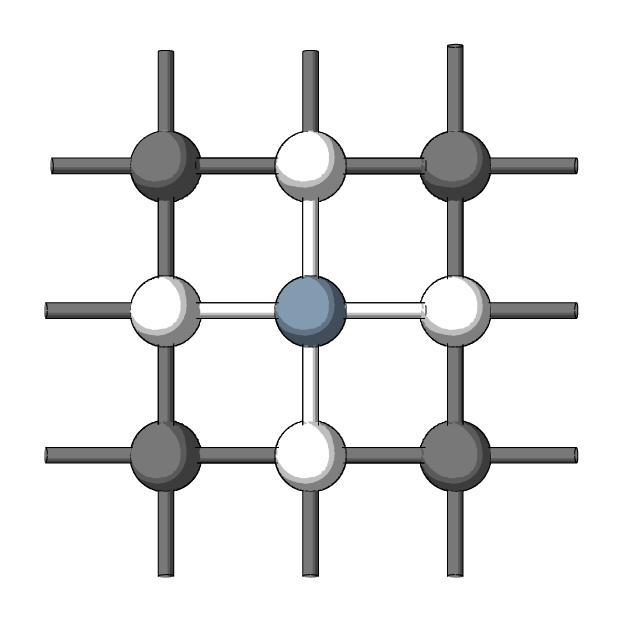
\includegraphics[width=0.48\columnwidth]{2dn4_lattice.png}
		\label{fig:lattice2dn4}
	}
	\subfigure[]
	{
		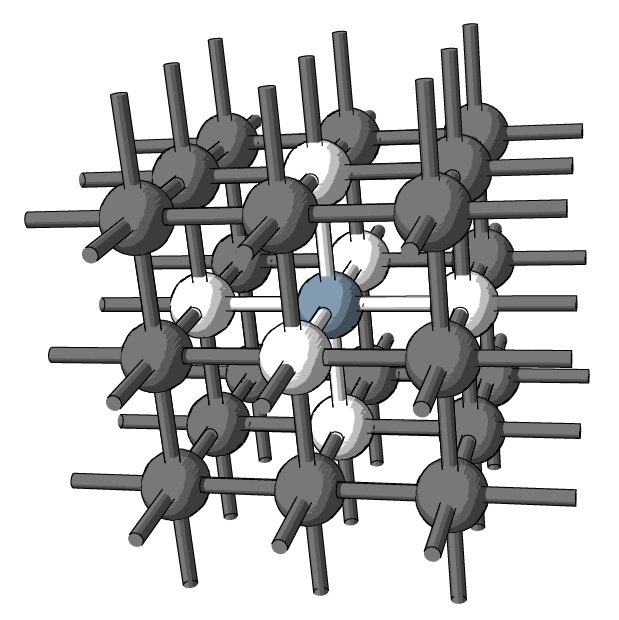
\includegraphics[width=0.48\columnwidth]{3dn6_lattice.png}
		\label{fig:lattice3dn6}
	}
	\caption{Common lattice structure for 2D and 3D image data. \textbf{(a)} Simplest connection of neighbouring pixels for 2D images. Each non-edge pixel is connected to 4 pixels. This is 4-connectedness. \textbf{(b)} Simplest connection of neighbouring voxels for 3D images. Each non-edge voxel is connected to 6 voxles. This is 6-connectedness.}
	\label{fig:connectedness}
\end{figure}

\begin{figure}[!t]
	\centering
	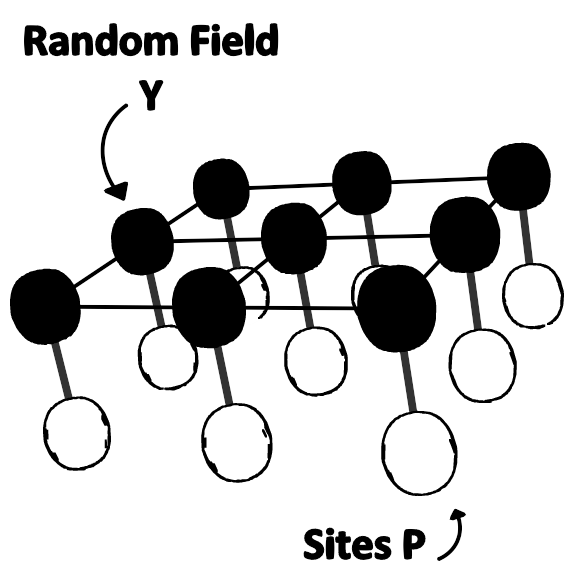
\includegraphics[width=0.35\columnwidth]{randomfield.png}
	\caption{4-connected random field $\mathbf{Y}$ over the sites $\mathcal{P}$.}
	\label{fig:randomfield}
\end{figure}

\begin{figure}[!t]
	\centering
	\subfigure[]
	{
		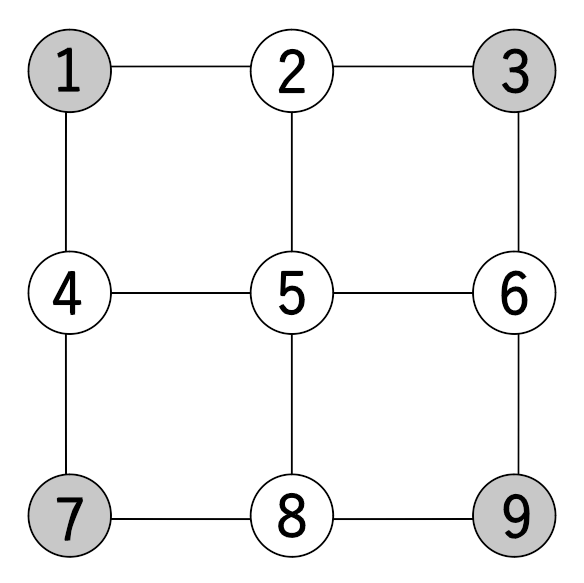
\includegraphics[width=0.35\columnwidth]{N4.png}
		\label{fig:n4}
	}
	\subfigure[]
	{
		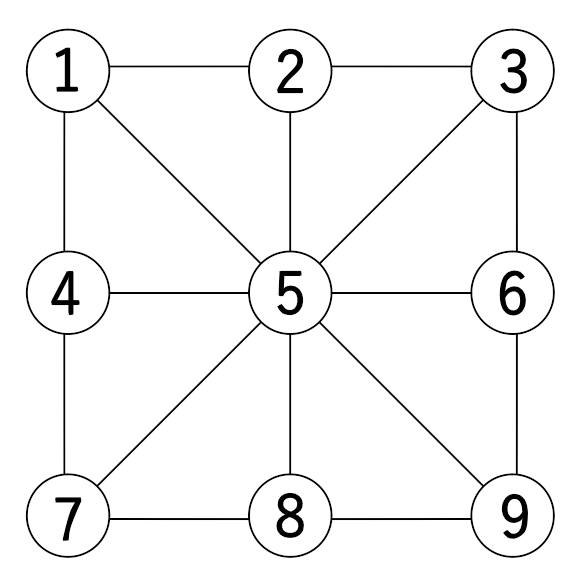
\includegraphics[width=0.35\columnwidth]{N8.png}
		\label{fig:n8}
	}
	\caption{Caption. \textbf{(a)} Caption. \textbf{(b)} Caption.}
	\label{fig:cliques}
\end{figure}

%----------------------------------------------------------------------------------------
%	SUBSECTION 2
%----------------------------------------------------------------------------------------

\subsection{MAP-MRF Estimation}
\label{sec:MAPMRFEstimation}

%----------------------------------------------------------------------------------------
%	SECTION 3
%----------------------------------------------------------------------------------------

\section{Graph Cuts}
\label{sec:GraphCuts}

%----------------------------------------------------------------------------------------
%	SUBSECTION 1
%----------------------------------------------------------------------------------------

\subsection{Network Theory and the Min-cut Problem}
\label{sec:NetworkTheory}

In this section we cover Graph Theory and specifically Flow Networks, which is a branch of Graph Theory, which is fundamental to the understanding of image segmentation via graph cuts. With it roots in Germany where Euler tried to find the solution to the Konigsberg bridge problem, graph theory has since blossomed into a rich field of Mathematics with seemingly endless amounts of application. Graph Theory is a huge topic in mathematics and can be applied to many other sciences. Graph theory is part of another more encompassing field of Mathematics known as Combinatronics. Graph theory and applications are more useful than the average person would recognise. They're used in Google Maps to find shortest routes to destinations, in Molecular Chemistry to model the structure of atoms, and the list goes on for quite a while. It is no surprise that it is also found to be useful in image segmentation.

\begin{definition}[Network]
	A network $N = (V,E)$ is a directed graph with a source node $s$, a sink node $t$ and a strictly positive capacity on every edge. That is, for each edge $e \in E$, the capacity, $c(.)$, obeys $c(e) \in \Re^{+}$.
\end{definition}

\tikzstyle{vertex}=[circle,thick,draw]
\tikzstyle{edge} = [draw=black!24, very thick,->]
\tikzstyle{weight} = [font=\small]
\begin{figure}[!h]
	\centering
	\resizebox {\columnwidth} {!} {
		\begin{tikzpicture}[scale=1.5, auto, swap, background rectangle/.style={fill=blue!10}, show background rectangle, >={Stealth[black!24]}]
		\draw[black] node at (-0.2,1.5) [font=\large,right,rounded corners,inner sep=1ex] {$\textbf{N}$};
		
		\draw node[circle,thick,right,fill=red!20,text=red!20] at (-0.2,0) {$s$};
		\draw node[circle,thick,right,fill=red!20,text=red!20] at (5.8,0) {$t$};
		\draw[dashed,draw=red!24,very thick] (0.0,0) -- (0.5,-1.5);
		\draw[dashed,draw=red!24,very thick] (6.0,0) -- (6.5,-1.5);
		\draw[dashed,draw=red!24,very thick] (2.65,1.25) -- (4,1.5);
		
		% draw the vertices
		\foreach \pos/\name in {{(0,0)/s},{(2,1)/a},{(4,1)/b},{(2,-1)/c},{(4,-1)/d}, {(6,0)/t}}
		\node[vertex] (\name) at \pos {$\name$};
		% connect vertices with edges and draw weights
		\foreach \source/ \dest /\weight in {s/a/7,s/c/2,a/b/{},c/d/2,b/t/5,d/t/3}
		\path[edge] (\source) edge node[weight] {$\weight$} (\dest);
		% bends
		\path [draw=black!24, very thick,->] (a) edge[bend left=-30] node {$3$} (d);
		\path [draw=black!24, very thick,->] (c) edge[bend left=30] node {$3$} (b);
		% info box		
		\draw node[circle,right,fill=red!20] at (2.65,1.25) {$5$};
		\draw node[right,rounded corners,fill=red!20,inner sep=1ex] at (4,1.5){$capacity$};
		\draw node[right,rounded corners,fill=red!20,inner sep=1ex] at (0,-1.5){$source$};
		\draw node[right,rounded corners,fill=red!20,inner sep=1ex] at (6,-1.5){$sink$};
		% s	
		\draw[orange] node at (-0.2,0.4) [font=\footnotesize,right,rounded corners,inner sep=1ex] {$d_{in}=0$};
		\draw[orange] node at (-0.2,0.7) [font=\footnotesize,right,rounded corners,inner sep=1ex] {$d_{out}=2$};	
		% t
		\draw[orange] node at (5.8,0.4) [font=\footnotesize,right,rounded corners,inner sep=1ex] {$d_{in}=2$};
		\draw[orange] node at (5.8,0.7) [font=\footnotesize,right,rounded corners,inner sep=1ex] {$d_{out}=0$};
		\end{tikzpicture}
	}
	\caption{Network \textbf{N} with no flow. The in-degree and out-degree for the source, \textbf{s}, and the sink, \textbf{t}, are shown next to the corresponding node.}
\end{figure}

The \textbf{source node} only has out-going edges, $d_{in}(s) = 0$ and $d_{out}(s) \geq 0$. The \textbf{sink node} only has incoming edges, $d_{in} \geq 0$ and $d_out = 0$.

\begin{definition}[Flow]
	A flow $f : V^2 \longrightarrow \Re^{+}$ is associated with each edge $e = (u,v)$ such that:
	\begin{enumerate}
		\item for each edge $e \in E$ we have $0 \leq f(e) \leq c(e)$. That is, the flow is positive and cannot excees the capacity of the edge.
		
		\item for each intermediate node $v \in V\setminus \{s,t\}$ the in- and out-flow of that node $\sum_{u \in V^-(v)} f(u,v) = \sum_{u \in V^+(v)} f(v,u)$.
	\end{enumerate}
\end{definition}

The \textbf{total flow} $F$ of a network is then what leave the source $s$ or reaches the sink $t$:
\begin{equation}
F(N) := \sum_{u \in V} f(s,u) - \sum_{u \in V}f(u,s) = \sum_{u \in V} f(u,t) - \sum_{u \in V}f(t,u)
\end{equation}

\tikzstyle{vertex}=[circle,thick,draw]
\tikzstyle{edge} = [draw=black!24, very thick,->]
\tikzstyle{weight} = [font=\small]
\begin{figure}[!h]
	\centering
	\resizebox {\columnwidth} {!} {
		\begin{tikzpicture}[scale=1.5, auto, swap, background rectangle/.style={fill=blue!10}, show background rectangle, >={Stealth[black!24]}]
		\draw[black] node at (-0.2,1.5) [font=\large,right,rounded corners,inner sep=1ex] {$\textbf{N}$};
		\draw node[circle,thick,right,fill=red!20,text=red!20] at (-0.2,0) {$s$};
		\draw node[circle,thick,right,fill=red!20,text=red!20] at (5.8,0) {$t$};
		\draw[dashed,draw=red!24,very thick] (2.65,1.25) -- (4,1.5);
		\draw[dashed,draw=red!24,very thick] (0.0,0) -- (0.5,-1.5);
		\draw[dashed,draw=red!24,very thick] (6.0,0) -- (6.5,-1.5);
		% draw the vertices
		\foreach \pos/\name in {{(0,0)/s},{(2,1)/a},{(4,1)/b},{(2,-1)/c},{(4,-1)/d}, {(6,0)/t}}
		\node[vertex] (\name) at \pos {$\name$};
		% connect vertices with edges and draw weights
		\foreach \source/ \dest /\weight in {s/a/{5/7},s/c/{2/2},a/b/{},c/d/{1/2},b/t/{4/5},d/t/{3/3}}
		\path[edge] (\source) edge node[weight] {$\weight$} (\dest);
		% bends
		\path [draw=black!24, very thick,->] (a) edge[bend left=-30] node {$1/3$} (d);
		\path [draw=black!24, very thick,->] (c) edge[bend left=30] node {$2/3$} (b);
		% info box		
		\draw node[rounded corners,right,fill=red!20] at (2.65,1.25) {$3/5$};
		\draw node[right,rounded corners,fill=red!20,inner sep=1ex] at (4,1.5){$flow/capacity$};
		% s	
		\draw node[right,rounded corners,fill=red!20,inner sep=1ex] at (0,-1.5) [font=\footnotesize,right,rounded corners,inner sep=1ex] {$\sum\limits_{u \in V_N} f(s,u)=7$};
		% t
		\draw node[right,rounded corners,fill=red!20,inner sep=1ex] at (6,-1.5) [font=\footnotesize,right,rounded corners,inner sep=1ex] {$\sum\limits_{u \in V_N} f(u,t)=7$};
		\end{tikzpicture}
	}
	\caption{Network \textbf{N} with flow. The flow out of the source node, \textbf{s}, is equal to the flow into the sink node, \textbf{t}. For all other nodes, the flow-in is equal to the flow-out. This is the conservation of flow principle. This is only part of the network. The remaining part is the residual graph which shows the amount of reverse flow is available on an edge.}
\end{figure}

\begin{definition}[Cut]
	A cut of a network $N = (V,E)$ is a partitioning of the vertex set $V = P \bigcup \bar{P}$ into two disjoint sets $P$ containining the source node $s$ and $\bar{P}$ containing the sink node $t$. $P \bigcap \bar{P} = \emptyset$.
\end{definition}

\tikzstyle{vertex}=[circle,thick,draw]
\tikzstyle{edge} = [draw=black!24, very thick,->]
\tikzstyle{weight} = [font=\small]
\begin{figure}[!h]
	\centering
	\resizebox {\columnwidth} {!} {
		\begin{tikzpicture}[scale=1.5, auto, swap, background rectangle/.style={fill=blue!10}, show background rectangle, >={Stealth[black!24]}]
		\draw[black] node at (-0.2,1.5) [font=\large,right,rounded corners,inner sep=1ex] {$\textbf{N}$};
		\path[fill=red!20,,use Hobby shortcut,closed=true] (-0.3,-0.1) .. (1,1) .. (2.3,1.2) .. (1.3,0.2);
		%		\draw node[text=blue] at (-0.3,0) {$1$};
		%		\draw node[text=blue] at (1,1) {$2$};
		%		\draw node[text=blue] at (2.5,1.2) {$3$};
		%		\draw node[text=blue] at (1,0.0) {$4$};
		\path[fill=blue!20,,use Hobby shortcut,closed=true] (1.5,-1) .. (2.5,0.5) .. (3.5,1.2) .. (5.2,1.0) .. (6.3,0.0) .. (5.0,-1);
		%		\draw node[text=blue] at (1,-1) {$1$};
		%		\draw node[text=blue] at (3.2,1.2) {$2$};
		%		\draw node[text=blue] at (5.0,1.2) {$3$};
		%		\draw node[text=blue] at (6.5,0.0) {$4$};
		% draw the vertices
		\foreach \pos/\name in {{(0,0)/s},{(2,1)/a},{(4,1)/b},{(2,-1)/c},{(4,-1)/d}, {(6,0)/t}}
		\node[vertex] (\name) at \pos {$\name$};
		% connect vertices with edges and draw weights
		\foreach \source/ \dest /\weight in {s/a/{},s/c/{},a/b/{},c/d/{},b/t/{},d/t/{}}
		{
			\path[edge] (\source) edge node[weight] {$\weight$} (\dest);
		}		
		% bends
		\path [draw=black!24,very thick,->,name path=curve1] (a) edge[bend left=-30] node {} (d);
		\path [draw=black!24,very thick,->,name path=curve2] (c) edge[bend left=30] node {} (b);
		% cut
		\draw node [text=orange] at (0,-0.7) {$C$};
		\path[dashed, very thick, draw=orange, name path=C] (0,-1) -- (3.5,1.5);
		% intersections
		\path [draw=black!24,name path=line1] (s) -- (c);		
		\path [draw=black!24,name path=line2] (a) -- (b);		
		\path [draw=blue!24,name path=line3] (a) edge [bend left=-30] (d);
		\fill [color=orange, name intersections={of=C and line1}] (intersection-1) circle (2pt);
		\fill [color=orange, name intersections={of=C and line2}] (intersection-1) circle (2pt);
		\fill [color=orange, name intersections={of=C and line3}] (2.15,0.53) circle (2pt);	
		% info box
		\draw[yshift=-2.1cm,xshift=-0.5cm]
		node [right,rounded corners,fill=orange!20,inner sep=1ex]
		{
			$S = \{s,a\}$, \, $T = \{t,b,c,d\}$, \,$C = \{(sc), (ab), (ad)\}$
		};
		\end{tikzpicture}
	}
	\caption{Network \textbf{N} with with a valid cut \textbf{C}. The nodes within the red region are reachable from the source and the nodes within the blue region are able to reach the sink. The cut set, \textbf{C}, is show in the orange filled block.}
\end{figure}

\tikzstyle{vertex}=[circle,thick,draw]
\tikzstyle{edge} = [draw=black!24, very thick,->]
\tikzstyle{weight} = [font=\small]
\begin{figure}[!h]
	\centering
	\resizebox {\columnwidth} {!} {
		\begin{tikzpicture}[scale=1.5, auto, swap, background rectangle/.style={fill=blue!10}, show background rectangle, >={Stealth[black!24]}]
		\draw[black] node at (-0.2,1.5) [font=\large,right,rounded corners,inner sep=1ex] {$\textbf{N}$};
		\path[fill=red!20,,use Hobby shortcut,closed=true] (-0.3,-0.1) .. (2,1.5) .. (4,1.5) .. (6.4,-0.1) .. (4,0) .. (2,0) ;
		%				\draw node[text=blue] at (-0.3,0) {$1$};
		%				\draw node[text=blue] at (2,1.5) {$2$};
		%				\draw node[text=blue] at (4,1.5) {$3$};
		%				\draw node[text=blue] at (6.3,0.0) {$4$};
		%				\draw node[text=blue] at (4,0.0) {$5$};
		%				\draw node[text=blue] at (2,0.0) {$6$};
		\path[fill=blue!20,,use Hobby shortcut,closed=true] (1.5,-1) .. (3.0,-0.7) .. (4.5,-1.0) .. (3.0,-1.2);
		%				\draw node[text=blue] at (1.5,-1) {$1$};
		%				\draw node[text=blue] at (3.0,-0.7) {$2$};
		%				\draw node[text=blue] at (4.5,-1.0) {$3$};
		%				\draw node[text=blue] at (3.0,-1.2) {$4$};			
		% draw the vertices
		\foreach \pos/\name in {{(0,0)/s},{(2,1)/a},{(4,1)/b},{(2,-1)/c},{(4,-1)/d}, {(6,0)/t}}
		\node[vertex] (\name) at \pos {$\name$};
		% connect vertices with edges and draw weights
		\foreach \source/ \dest /\weight in {s/a/{},s/c/{},a/b/{},c/d/{},b/t/{},d/t/{}}
		{
			\path[edge] (\source) edge node[weight] {$\weight$} (\dest);
		}		
		% bends
		\path [draw=black!24,very thick,->,name path=curve1] (a) edge[bend left=-30] node {} (d);
		\path [draw=black!24,very thick,->,name path=curve2] (c) edge[bend left=30] node {} (b);
		% cut
		\draw node [text=orange] at (0,-0.7) {$C$};
		\path[dashed, very thick, draw=orange, name path=C] (0,-1) edge[bend left=30] (6,-1);
		% intersections
		\fill [color=orange] (1.0,-0.5) circle (2pt);
		\fill [color=orange] (5.0,-0.5) circle (2pt);
		\fill [color=orange] (2.28,-0.18) circle (2pt);
		\fill [color=orange] (2.52,-0.165) circle (2pt);
		% info box
		%		\draw[yshift=-2.1cm,xshift=-0.5cm]
		%		node [right,rounded corners,fill=orange!20,inner sep=1ex]
		%		{
		%			$S = \{s,a\}$, \, $T = \{t,b,c,d\}$, \,$C = \{(sc), (ab), (ad)\}$
		%		};
		\end{tikzpicture}
	}
	\caption{Network \textbf{N} with with a invalid cut \textbf{C}. The cut does not partition source node \textbf{s} and sink node \textbf{t} into distinct sets.}
\end{figure}

\tikzstyle{vertex}=[circle,thick,draw]
\tikzstyle{edge} = [draw=black!24, very thick,->]
\tikzstyle{weight} = [font=\small]
\begin{figure}[!h]
	\centering
	\resizebox {\columnwidth} {!} {
		\begin{tikzpicture}[scale=1.5, auto, swap, background rectangle/.style={fill=blue!10}, show background rectangle, >={Stealth[black!24]}]
		\draw[black] node at (-0.2,1.5) [font=\large,right,rounded corners,inner sep=1ex] {$\textbf{N}$};
		%		\path[fill=red!20,,use Hobby shortcut,closed=true] (-0.3,-0.1) .. (2,1.5) .. (4,1.5) .. (6.4,-0.1) .. (4,0) .. (2,0) ;
		%				\draw node[text=blue] at (-0.3,0) {$1$};
		%				\draw node[text=blue] at (2,1.5) {$2$};
		%				\draw node[text=blue] at (4,1.5) {$3$};
		%				\draw node[text=blue] at (6.3,0.0) {$4$};
		%				\draw node[text=blue] at (4,0.0) {$5$};
		%				\draw node[text=blue] at (2,0.0) {$6$};
		%		\path[fill=blue!20,,use Hobby shortcut,closed=true] (1.5,-1) .. (3.0,-0.7) .. (4.5,-1.0) .. (3.0,-1.2);
		%				\draw node[text=blue] at (1.5,-1) {$1$};
		%				\draw node[text=blue] at (3.0,-0.7) {$2$};
		%				\draw node[text=blue] at (4.5,-1.0) {$3$};
		%				\draw node[text=blue] at (3.0,-1.2) {$4$};			
		% draw the vertices
		\foreach \pos/\name in {{(0,0)/s},{(2,1)/a},{(4,1)/b},{(2,-1)/c},{(4,-1)/d}, {(6,0)/t}}
		\node[vertex] (\name) at \pos {$\name$};
		% connect vertices with edges and draw weights
		\foreach \source/ \dest /\weight in {s/a/{},s/c/{},a/b/{},c/d/{},b/t/{},d/t/{}}
		{
			\path[edge] (\source) edge node[weight] {$\weight$} (\dest);
		}		
		% bends
		\path [draw=black!24,very thick,->,name path=curve1] (a) edge[bend left=-30] node {} (d);
		\path [draw=black!24,very thick,->,name path=curve2] (c) edge[bend left=30] node {} (b);
		% cut
		\draw node [text=orange] at (0,-0.7) {$C$};
		\draw [dashed, orange, very thick] plot [smooth] coordinates {(0,-1) (2.5,1) (3,1.2) (3.5,-1.5)};
		% intersections
		\fill [color=orange] (0.77,-0.37) circle (2pt);
		\fill [color=orange] (2.09,0.68) circle (2pt);
		\fill [color=orange] (2.5,1) circle (2pt);
		\fill [color=orange] (3.05,1) circle (2pt);
		\fill [color=orange] (3.12,0.7) circle (2pt);
		\fill [color=orange] (3.40,-0.82) circle (2pt);
		\fill [color=orange] (3.42,-1) circle (2pt);
		% info box
		%		\draw[yshift=-2.1cm,xshift=-0.5cm]
		%		node [right,rounded corners,fill=orange!20,inner sep=1ex]
		%		{
		%			$S = \{s,a\}$, \, $T = \{t,b,c,d\}$, \,$C = \{(sc), (ab), (ad)\}$
		%		};
		\end{tikzpicture}
	}
	\caption{Network \textbf{N} with with a invalid cut \textbf{C}. The cut partition partitions the graph into more than two sets and the cut intersects the edges $ab$ and $ad$ twice.}
\end{figure}

The \textbf{capacity} of a cut is the sum of the edges $(u,v) \in V$ where $u \in P$ and $v \in \bar{P}$:
\begin{equation}
\kappa (P, \bar{P}) = \sum_{u \in P; v \in \bar{P}} c(u,v)
\end{equation}

\begin{definition}[Maximal Flow]
	The largest amount of flow that can be sent through the source that is able to reach the sink is known as the maximal flow.
\end{definition}

\tikzstyle{vertex}=[circle,thick,draw]
\tikzstyle{edge} = [draw=black!24, very thick,->]
\tikzstyle{weight} = [font=\small]
\begin{figure}[!h]
	\centering
	\resizebox {\columnwidth} {!} {
		\begin{tikzpicture}[scale=1.5, auto, swap, background rectangle/.style={fill=blue!10}, show background rectangle, >={Stealth[black!24]}]
		\draw[black] node at (-0.2,1.5) [font=\large,right,rounded corners,inner sep=1ex] {$\textbf{N}$};
		\draw node[circle,thick,right,fill=red!20,text=red!20] at (-0.2,0) {$s$};
		\draw node[circle,thick,right,fill=red!20,text=red!20] at (5.8,0) {$t$};
		\draw[dashed,draw=red!24,very thick] (0.0,0) -- (0.5,-1.5);
		\draw[dashed,draw=red!24,very thick] (6.0,0) -- (6.5,-1.5);
		% draw the vertices
		\foreach \pos/\name in {{(0,0)/s},{(2,1)/a},{(4,1)/b},{(2,-1)/c},{(4,-1)/d}, {(6,0)/t}}
		\node[vertex] (\name) at \pos {$\name$};
		% connect vertices with edges and draw weights
		\foreach \source/ \dest /\weight in {s/a/{6/7},s/c/{2/2},a/b/{5/5},c/d/{2/2},b/t/{5/5},d/t/{3/3}}
		\path[edge] (\source) edge node[weight] {$\weight$} (\dest);
		% bends
		\path [draw=black!24, very thick,->] (a) edge[bend left=-30] node {$0/3$} (d);
		\path [draw=black!24, very thick,->] (c) edge[bend left=30] node {$1/3$} (b);
		%info
		% s	
		\draw node[right,rounded corners,fill=red!20,inner sep=1ex] at (0,-1.5) [font=\footnotesize,right,rounded corners,inner sep=1ex] {$\sum\limits_{u \in V_N} f(s,u)=8$};
		% t
		\draw node[right,rounded corners,fill=red!20,inner sep=1ex] at (6,-1.5) [font=\footnotesize,right,rounded corners,inner sep=1ex] {$\sum\limits_{u \in V_N} f(u,t)=8$};
		\end{tikzpicture}
	}
	\caption{Network \textbf{N} with maximum flow. There is no way to push more flow out of the source into the sink without breaking the rules for conservation of flow.}
\end{figure}

\begin{definition}[Minimal Cut]
	A cut $C$ on a network $N = (V,E)$ is a minimal cut if there exists no other cut $C'$ where $\kappa (C') < \kappa(C)$.
\end{definition}

\tikzstyle{vertex}=[circle,thick,draw]
\tikzstyle{edge} = [draw=black!24,very thick,->]
\tikzstyle{weight} = [font=\small]
\begin{figure}[!h]
	\centering
	\resizebox {\columnwidth} {!} {
		\begin{tikzpicture}[scale=1.5, auto, swap, background rectangle/.style={fill=blue!10}, show background rectangle, >={Stealth[black!24]}]
		\draw[black] node at (-0.2,1.5) [font=\large,right,rounded corners,inner sep=1ex] {$\textbf{N}$};	
		\path[fill=red!20,,use Hobby shortcut,closed=true] (-0.3,-0.1) .. (2,1.5) .. (4,1.5) .. (4.5,-0.1) .. (4,-1.5) .. (2,-1.5) ;
		%			\draw node[text=blue] at (-0.3,0) {$1$};
		%			\draw node[text=blue] at (2,1.5) {$2$};
		%			\draw node[text=blue] at (4,1.5) {$3$};
		%			\draw node[text=blue] at (6.3,0.0) {$4$};
		%			\draw node[text=blue] at (4,-1.5) {$5$};
		%			\draw node[text=blue] at (2,-1.5) {$6$};
		\path[fill=blue!20,use Hobby shortcut,closed=true] (5.5,0) .. (6.0,0.5) .. (6.5,0) .. (6.0,-0.5);
		%			\draw node[text=blue] at (5.5,0) {$1$};
		%			\draw node[text=blue] at (6.0,0.5) {$2$};
		%			\draw node[text=blue] at (6.5,0) {$3$};
		%			\draw node[text=blue] at (6.0,-0.5) {$4$};
		% draw the vertices
		\foreach \pos/\name in {{(0,0)/s},{(2,1)/a},{(4,1)/b},{(2,-1)/c},{(4,-1)/d}, {(6,0)/t}}
		\node[vertex] (\name) at \pos {$\name$};
		% connect vertices with edges and draw weights
		\foreach \source/ \dest /\weight in {s/a/7,s/c/2,a/b/{5},c/d/2,b/t/5,d/t/3}
		\path[edge] (\source) edge node[weight] {$\weight$} (\dest);
		% bends
		\path [draw=black!24, very thick,->] (a) edge[bend left=-30] node {$3$} (d);
		\path [draw=black!24, very thick,->] (c) edge[bend left=30] node {$3$} (b);
		% cut
		\draw node [text=orange] at (4.8,-1.0) {$C$};
		\path[dashed, very thick, draw=orange, name path=C] (5,-1.2) -- (5,1.2);
		% intersections
		\path [draw=black!24,name path=line1] (b) -- (t);
		\path [draw=black!24,name path=line2] (d) -- (t);
		\fill [color=orange, name intersections={of=C and line1}] (intersection-1) circle (2pt);
		\fill [color=orange, name intersections={of=C and line2}] (intersection-1) circle (2pt);
		%info
		% minimum capacity	
		\draw node[right,rounded corners,fill=orange!20,inner sep=1ex] at (5,-1.5) [font=\footnotesize,right,rounded corners,inner sep=1ex] {$\sum\limits_{e \in C} c(e)=8$};
		\end{tikzpicture}
	}
	\caption{Network \textbf{N} with minimal cut \textbf{C}. The sum of the capacity of all the edges in the cut set is the minimum of all possible valid cuts on the network \textbf{N}.}
\end{figure}

In the next section we show that the Maximal Flow problem and the Minimal Cut problem are duals of each other, commonly known as the Max-Flow/Min-Cut problem.

%----------------------------------------------------------------------------------------
%	SUBSECTION 2
%----------------------------------------------------------------------------------------

\subsection{Image Segmentation Framework/Graph Construction Images}
\label{sec:GraphCutFramework}

%----------------------------------------------------------------------------------------
%	SECTION 4
%----------------------------------------------------------------------------------------

\section{Energy Minimisation}
\label{sec:EnergyMinimisation}

%----------------------------------------------------------------------------------------
%	SUBSECTION 1
%----------------------------------------------------------------------------------------

\subsection{General Form of Energy Functions}
\label{sec:GeneralEnergyFunctions}

%----------------------------------------------------------------------------------------
%	SUBSECTION 2
%----------------------------------------------------------------------------------------

\subsection{Submodular Functions}
\label{sec:Submodular Functions}

%----------------------------------------------------------------------------------------
%	SECTION 3
%----------------------------------------------------------------------------------------

\subsection{Energy Minimisation Algorithms}
\label{sec:MaxFlowMinCutAlgoithms}

Lorem ipsum dolor sit amet, consectetur adipiscing elit. Aliquam ultricies lacinia euismod. Nam tempus risus in dolor rhoncus in interdum enim tincidunt. Donec vel nunc neque. In condimentum ullamcorper quam non consequat. Fusce sagittis tempor feugiat. Fusce magna erat, molestie eu convallis ut, tempus sed arcu. Quisque molestie, ante a tincidunt ullamcorper, sapien enim dignissim lacus, in semper nibh erat lobortis purus. Integer dapibus ligula ac risus convallis pellentesque.

%-----------------------------------
%	SUBSECTION 1
%-----------------------------------
\subsubsection{Ford-Fulkerson}

Nunc posuere quam at lectus tristique eu ultrices augue venenatis. Vestibulum ante ipsum primis in faucibus orci luctus et ultrices posuere cubilia Curae; Aliquam erat volutpat. Vivamus sodales tortor eget quam adipiscing in vulputate ante ullamcorper. Sed eros ante, lacinia et sollicitudin et, aliquam sit amet augue. In hac habitasse platea dictumst.

\begin{algorithm}
	\caption{Euclid’s algorithm}\label{alg:euclid}
	\begin{algorithmic}[1]
		\Procedure{Euclid}{$a,b$}\Comment{The g.c.d. of a and b}
		\State $r\gets a\bmod b$
		\While{$r\not=0$}\Comment{We have the answer if r is 0}
		\State $a\gets b$
		\State $b\gets r$
		\State $r\gets a\bmod b$
		\EndWhile\label{euclidendwhile}
		\State \textbf{return} $b$\Comment{The gcd is b}
		\EndProcedure
	\end{algorithmic}
\end{algorithm}

%-----------------------------------
%	SUBSECTION 2
%-----------------------------------

\subsubsection{Dinic/Edmond-Karp}
Morbi rutrum odio eget arcu adipiscing sodales. Aenean et purus a est pulvinar pellentesque. Cras in elit neque, quis varius elit. Phasellus fringilla, nibh eu tempus venenatis, dolor elit posuere quam, quis adipiscing urna leo nec orci. Sed nec nulla auctor odio aliquet consequat. Ut nec nulla in ante ullamcorper aliquam at sed dolor. Phasellus fermentum magna in augue gravida cursus. Cras sed pretium lorem. Pellentesque eget ornare odio. Proin accumsan, massa viverra cursus pharetra, ipsum nisi lobortis velit, a malesuada dolor lorem eu neque.

%-----------------------------------
%	SUBSECTION 3
%-----------------------------------

\subsubsection{Push-Relabel}
Originally developed by Andrew V. Goldberg and Robert E. Tarjan. Previous algorithms, such as Ford-Fulkerson, used the concept of residual networks and augmenting paths to determine max-flow.
Push-Relabel used the concept of preflow to determine  max-flow instead of augmenting paths. Sometimes referred as the Preflow-Push Algorithm.
Preflow is a concept originally developed by A.V. Karzanov.

The algorithm works at converting a preflow, $f$, into a normal flow and then terminates. This flow also turns out to be the maximum flow. Goldberg and Tarjan defined a generic Push-Relabel algorithm  which solves the maximum flow problem.

\begin{definition}[Preflow]
	A preflow is a real-valued function, $f$, on vertice pairs. The total flow into a vertex can exceed the flow out of a vertex but not vice versa.
\end{definition}
A preflow where all $v \in V-\{s, t\}$ has a flow excess of zero, $e_f(v) = 0$, is a normal flow. The preflow function is also referred to as the \textbf{s-t preflow}.

Preflow must satisfy:
\begin{enumerate}
	\item Capacity Constraint\\
	$\forall u,v \in V, f(u,v) \leq c(u,v)$
	
	\item Antisymmetry/Skew Symmetry\\
	$\forall u, v, \in V, f(u,v) = -f(v,u)$
	
	\item Nonnegative Constrain\\
	The flow into $v \in V-\{s\}$ must be greater than or equal to the flow out of $v$. $\forall u \in V, v \in V-\{s\}, \sum f(u,v)>0$
\end{enumerate}

\begin{definition}[Flow Excess]
	Flow excess, $e_f(v)$, is the net flow into $v$ where $v \in V$ for some preflow $f$.
\end{definition}

\[
e_f(v) =
\begin{cases} 
\hfill \infty \hfill & \text{ if $v=s$} \\
\hfill \sum_{u \in V}f(u,v) \hfill & \text{ if $v \in V-\{s\}$} \\
\end{cases}
\]

\begin{definition}[Active Vertex]
	An active vertex/node is a vertex $v$ which satisfies all of the properties:
	\begin{enumerate}
		\item Not a source or sink, $v \in V-\{s,t\}$
		\item Positive flow excess, $e_f(v) > 0$
		\item Has a valid label, $d(v) < \infty$
	\end{enumerate}
\end{definition}

Push-Relabel also uses the concept of a residual graph, $G_f=(V, E_f)$.

\begin{definition}[Residual Capacity]
	The residual capacity of a preflow is defined as $r_f(v,w) = c(v,w)-f(v,w)$.
\end{definition}

\begin{definition}[Residual Edges]
	The residual edges for a preflow $f$ is defined as the set of edges with positive residual capacity. $E_f = \{(v,w)\} | r-f(v,w) > 0$.
\end{definition}

\begin{definition}[Labelling]
	Push-Relabel also use a valid labelling function, $d$, to determine which vertex pairs should be selected for the push operation.
\end{definition}
A valid labelling , $d$, is a nonnegative integer function applied to all vertices to denote a label. The labelling is often referred as the height or distance from the sink node, $t$. This function is sometimes compared to the physical intuition that liquids naturally flow downhill.

A valid labelling for a preflow consists of:
\begin{enumerate}
	\item For $v \in V, 0 \leq d(v) \leq \infty$
	\item $d(s) = |V| \text{ (source condition)}$
	\item $d(t) = 0 \text{ (sink condition)}$
	\item $d(v) = d(w) + 1$ for every residual edge $(v,u) \in E_f$
\end{enumerate}
A labelling $d$ and a preflow $f$ are said to be compatible id $d$ adheres to the properties above.

The algorithm pushes flow excess starting at the source, $s$, along all vertices towards the sink, $t$. The algorithm maintains a compatible vertex labelling function, $d$, to the preflow, $f$. The labelling is usedto determine where to puch the flow excess. The algorithm repeatedly performs either a push or a relabel operation so long as there is an active vertex in $G_f$.

\begin{definition}[Push Operation]
	The push operation is used to move flow from one vertex to another. The transfer of excess can be performed across the vertex pair $(v,w) \in E_f$ if:
	\begin{enumerate}
		\item $v$ is an active vertex
		\item the edge has positive residual capacity, $r_f(v,w)>0$
		\item the label distance $d(v) = d(w)+1$
	\end{enumerate}
\end{definition}
This allows the algorithm to move $\delta$ excess flow: $\delta = min (e_f(v), r_f(v,w))$ from $v$ to $w$. A push is considered \textbf{saturating} if no more flow can be sent over the edge, $\delta = r_f(v,w)$. A push is considered to be \textbf{non-saturating} if all the excess from $v$ the push over the dge and the edge still has some cpacity, $\delta = e_f(v)$.

\begin{algorithm}
	\caption{Push Operation}\label{alg:push}
	\textbf{Input:} Preflow $f$, labels $d$, and $(v,w)$ where $v,w \in V$\\
	\textbf{Output:} Preflow $f$\\
	\textbf{Applicable:} if $v \in V-\{s,t\}$, $d(v) < \infty$, $e_f(v)>0$, $r_f(v,w)>0$ and $d(v)=d(w)+1$
	\begin{algorithmic}[1]
		\Procedure{Push}{$v,w$}
		\State $\delta \coloneqq min(e_f(v), r_f(v,w)$
		\State $f(v,w) \coloneqq f(v,w) + \delta$
		\State $f(w,v) \coloneqq f(w,v) - \delta$
		\State $e_f(v) \coloneqq e_f(v) - \delta$
		\State $e_f(w) \coloneqq e_f(w) + \delta$
		\State \textbf{return} $f$
		\EndProcedure
	\end{algorithmic}
\end{algorithm}
	
\begin{definition}[Relabel Operation]
	The relabel operation is used to increase the label value of a single active vertex so that excess flow can be pushed out of the active vertex. The relabel operation is performed when all the residual edges of the active vertex have positive residual capacity, $r_f(v,w)>0$. This implies that $v$'s label is less than or equal to all vertices, $d(v) \leq d(w)$, meaning that no push operation across the edges is possible given the push condition $d(v) = d(w)+1$.
\end{definition}
The relabel operation for some vertex $v$ selects the smallest label for the vertices with positive residual edges, $r_f(v,w)>0$. The active vertex is then assigned the smallest label value $+1$ such that $d(v) := min{d(v)+1 | (v,w) \in E_f}$. This will alow the vertex $v$ to potentially push its excess flow to atleast one of the othe vertices during the algorithm's next iteration.

\begin{algorithm}
	\caption{Relabel Operation}\label{alg:relabel}
	\textbf{Input:} Preflow $f$, labels $d$, and $v \in V-\{s,t\}$\\
	\textbf{Output:} Labels $d$\\
	\textbf{Applicable:} if $v \in V-\{s,t\}$, $d(v) < \infty$, $e_f(v)>0$, and $\forall w \in V, r_f(v,w)>0$ which implies $d(v) \leq d(w)$
	\begin{algorithmic}[1]
		\Procedure{Relabel}{$v$}
		\If {$\{(v,w) \in E_f\} \neq 0$}
		\State $d(v) \coloneqq min(d(w)+1 | (v,w) \in E_f)$
		\Else 
		\State $d(v) \coloneqq \infty$
		\EndIf
		\State \textbf{return} $d$
		\EndProcedure
	\end{algorithmic}
\end{algorithm}

The algorithm initialises the following values in the residual graph before the push andrelabel operations in the main loop.
\begin{enumerate}
	\item Initialise the preflow of all edges in the  residual graph
	
	\item Initialise the labellings such that:
	\begin{enumerate}
		\item $d(s) = |V|$
		\item $d(v) = 0 \text{for } v \in V-\{s\}$
	\end{enumerate}
	
	\item Performs saturation, pushes along all residual edges out of the source $(s,v) \in E_f$ and $v \in V$.
\end{enumerate}
Once complete the algorithm repeatedly performs either a push or a relabel operation against all vertices. The algorithm continues until no operation can be performed. The algorithm terminates when there are no more active vertices.

\begin{algorithm}
	\caption{Push-Relabel Main-loop}\label{alg:main_no_optimisation}
	\textbf{Input:} Network flow graph $G=(V,E)$, $s$, $t$ and $c$\\
	\textbf{Output:} Maximum flow $f$
	\begin{algorithmic}[1]
		\Procedure{Main}{$v$}
		\ForAll {$(v,w) \in (V-\{s\})(V-\{s\})$}
		\State $f(v,w) \gets 0$
		\State $f(w,v) \gets 0$
		\EndFor
		\item[]
		\ForAll {$v \in V$}
		\State $f(s,v) \gets r_f(s,v)$
		\State $f(v,s) \gets -r_f(s,v)$
		\EndFor
		\item[]
		\State $d(s) \gets |V|$
		\item[]
		\ForAll {$v \in V-\{s\}$}
		\State $d(v) \gets 0$
		\State $e_f(v) \gets f(s,v)$
		\EndFor
		\item[]
		\State While there exists an active vertex
		\While {$\exists v \in V-\{s,t\}$} \Comment{with either applicable PUSH() or RELABEL() operation}
		\State Perform either a PUSH or a RELABEL operation on $v$
		\EndWhile
		\item[]
		\State \textbf{return} $f$
		\EndProcedure
	\end{algorithmic}
\end{algorithm}

The analaysis and the proof of correctness of the Push-Relabel algorithm can be found in \autoref{AppendixB}.

%-----------------------------------
%	SUBSUBSECTION 1
%-----------------------------------

\subsubsection{Push-Relabel Speed Optimisation Heuristics}
\begin{definition}[Discharge]
	Push-Relabel also use a valid labelling function ,$d$, to determine which vertex pairs should be selected for the push operation.
\end{definition}

\begin{definition}[FIFO]
	Push-Relabel also use a valid labelling function ,$d$, to determine which vertex pairs should be selected for the push operation.
\end{definition}

\begin{definition}[Highest Label First]
	Push-Relabel also use a valid labelling function ,$d$, to determine which vertex pairs should be selected for the push operation.
\end{definition}

\begin{definition}[Global Relabel]
	Push-Relabel also use a valid labelling function ,$d$, to determine which vertex pairs should be selected for the push operation.
\end{definition}

\begin{definition}[Gap Relabel]
	Push-Relabel also use a valid labelling function ,$d$, to determine which vertex pairs should be selected for the push operation.
\end{definition}
